\documentclass[]{gshs_exam} %XeLaTeX로 조판

% 필요한 패키지는 여기에 작성하세요
\usetikzlibrary{patterns,decorations.pathmorphing,decorations.markings}
\tikzset{middlearrow/.style=
  {decoration={markings,mark=at position 0.6 with {\arrow{latex}}}, postaction={decorate}
}}
\usepackage{bm}
\usepackage{tikz-3dplot}
\usepackage{circuitikz}
\usepackage{mathrsfs} 
\usepackage[export]{adjustbox}
%



\makeatletter
\myyear{2018}\let\MyYear\@myyear %학년도
\semester{1}\let\Semester\@semester %학기
\exams{1차 지필평가}\let\Exams\@exams %1차,2차 지필평가
\subject{일반물리학I}\let\Subject\@subject %과목명
\credits{3} %학점
\pfscore{100} %만점
\examtime{60분} %시험시간
\numexaminers{4} %출제인원 (1~4 중 하나를 입력)
\examiner{홍길동} %출제1
\examinerII{홍동길} %출제2
\examinerIII{길홍동}%출제3
\examinerIV{동홍길}%출제4
\reviewer{허\hspace{1em}균} %검토
\makeatother

%% 한글줄간격 %% 영어로 작성한 경우 아랫줄을 주석 처리한다.
\renewcommand{\baselinestretch}{1.3}


\begin{document}
\maketitle


%%% page 1 %%%
\begin{multicols*}{2} % 다단(2단) 페이지 시작
\noindent\fbox{\parbox{0.98\columnwidth}{\vspace*{-0.6em}
\begin{enumerate}[leftmargin=5.5mm,label=※]
\item 문항에 따라 배점이 다르므로 각 물음의 끝에 표시된 배점을 참고하시오.\\[-2.2em]
\item 단답형 ( 18 )점, 서술형 ( 67 )점, 논술형 ( 15 )점
\end{enumerate}\vspace{-0.6em}}}\vspace{1em}

\begin{questions} % 문항 환경 시작

%% 문항은 \question이란 명령어를 사용한다.
%% 굵은 글자의 [단답형], [서술형], [논술형] 표기는 각각 \ddh\ , \ssh\ , \nsh\ 이란 명령어로 정의해 두었다.
\question \ddh\ 그림은 두께를 무시할 수 있는 균일한 금속판으로 만든 정육면체 상자이다. 상자의 위쪽은 열려 있고 한 변의 길이는 $L$이다. 상자 질량중심의 좌표를 구하시오.  [8점]

\begin{center} % 중앙 정렬
\def\al{65}\def\be{115}
\tdplotsetmaincoords{\al}{\be}
\begin{tikzpicture}[tdplot_main_coords] % 그림 그리기
\small
\def\L{2}\def\t{0.08}
\draw[-latex] (0,0,0) -- ({1.5*\L},0,0) node[pos=1,left]{$x$};
\draw[-latex] (0,0,0) -- (0,{1.5*\L},0) node[pos=1,right]{$y$};
\draw[-latex] (0,0,0) -- (0,0,{1.5*\L}) node[pos=1,left]{$z$};
\draw[fill=black!15] (\t,\t,\t) -- (\t,\t,\L) -- ({\L-\t},\t,\L) -- ({\L-\t},\t,\t) -- cycle;
\draw[fill=black!5] (\t,\t,\t) -- (\t,{\L-\t},\t) -- (\t,{\L-\t},\L) -- (\t,\t,\L) -- cycle;
\fill[white] (0,0,\L) -- (\L,0,\L) -- (\L,\L,\L) -- ({\L-\t},\L,\L) -- ({\L-\t},\t,\L) -- (0,\t,\L) -- cycle;
\fill[white] (0,0,\L) -- (0,\L,\L) -- (\L,\L,\L) -- (\L,{\L-\t},\L) -- (\t,{\L-\t},\L) -- (\t,0,\L) -- cycle;
\draw[join=bavel,fill=black!3] (\L,0,0) -- ++(0,\L,0) -- ++(0,0,\L) -- ++(0,-\L,0) -- cycle;
\draw[join=bavel,fill=black!10] (0,\L,0) -- ++(\L,0,0) -- ++(0,0,\L) -- ++(-\L,0,0) -- cycle;
\draw[join=bavel] (\L,0,\L) -- (0,0,\L) -- (0,\L,\L);
\draw[join=bavel] (\t,\t,\L) -- ({\L-\t},\t,\L) -- ({\L-\t},{\L-\t},\L) -- (\t,{\L-\t},\L) -- cycle;
\end{tikzpicture} % 그림 그리기 종료
\end{center} % 중앙 정렬 종료

\vspace{10em}

\question \ssh\ 그림처럼 질량 $M$인 토막이 마찰이 없는 수평면 위에 놓여 있고, 그 위에 질량 $m$인 토막이 놓여 있다. 토막 사이의 정지마찰계수는 $\mu_\mathrm{k}$이고, 아래 토막에 연결된 용수철의 용수철 상수는 $k$이다. 위 토막이 미끄러지지 않도록 하는 진폭의 최댓값을 구하시오. [12점]

\begin{center}
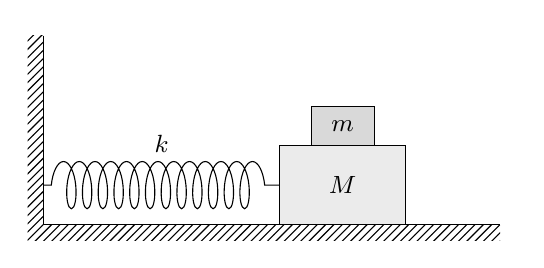
\begin{tikzpicture}\small
\fill[pattern=north east lines] (-0.2,-0.2) rectangle (5.8,2.4);
\fill[white] (0,0) rectangle (6,2.5);
\draw (0,2.4) -- (0,0) -- (5.8,0);
\draw[fill=black!8] (3,0) rectangle ++(1.6,1) node[pos=0.5]{$M$};
\draw[fill=black!15] (3.4,1) rectangle ++(0.8,0.5) node[pos=0.5]{$m$};
\draw[decorate,decoration={coil,amplitude=0.3cm,segment length=0.2cm,pre length=0.1cm,post length=0.1cm,aspect=0.35}] (0,0.5) -- (3,0.5) node[pos=0.5,above=0.3cm]{$k$};
\end{tikzpicture}
\end{center}

\vspace*{\fill} % 다음 단(column)으로 이동하기 전 현재 column을 여백으로 채움
\columnbreak % 현재 column에서의 작성 종료

\question 그림은 선밀도 $\mu$, 길이 $L$의 팽팽한 줄에 질량 $m$인 물체와 진동자가 연결된 것을 나타낸 것이다. 점 P를 통해 진동수 $f$의 조화파동이 만들어지고, 고정된 점 Q에서 파동이 반사된다. 점 P와 Q에서의 진폭은 미미하므로 각각 마디로 볼 수 있다. (단, 중력가속도는 $g$이다.) [총 17점]
\begin{center}
\begin{tikzpicture}\small
\draw[fill=black!5] (0,-0.4) rectangle (1.1,0.4) node[pos=0.5]{진동자};
\draw[thick] (1.1,0) -- (6,0) arc (90:0:0.06) -- (6.06,-1.5);
\draw[thick,opacity=0.4] (1.4,0) sin ++({4.6/6},0.4) cos ++({4.6/6},-0.4) sin ++({4.6/6},-0.4) cos ++({4.6/6},0.4) sin ++({4.6/6},0.4) cos ++({4.6/6},-0.4);
\draw[thick,opacity=0.4] (1.4,0) sin ++({4.6/6},-0.4) cos ++({4.6/6},0.4) sin ++({4.6/6},0.4) cos ++({4.6/6},-0.4) sin ++({4.6/6},-0.4) cos ++({4.6/6},0.4);
\fill[black] (1.4,0) circle (0.06) node[above=0.06]{P};
\fill[black] (6,-0.06) circle (0.06) node[above=0.06]{Q};
\draw[thin] (1.4,0) -- (1.4,-1.2);
\draw[thin] (6,-0.06) -- (6,-1.2);
\draw[latex-latex] (1.4,-0.8) -- (6,-0.8) node[fill=white,pos=0.5]{$L$};
\draw[fill=black!15] ({6.06-0.5},-1.5) rectangle ({6.05+0.5},-2.5) node[pos=0.5] {$m$};
\end{tikzpicture}
\end{center}
%% 소문항은 parts환경에서 작성한다.
%% 즉 \begin{parts} 와 \end{parts} 사이에 작성한다.
%% 소문항의 명령어는 \part이다.
\begin{parts}
\part \ddh\ 줄에 3차 화음을 만드는 질량 $m$을 구하시오. [6점]
\vspace{10em}
\part \ssh\ 질량이 $2$배인 물체를 매달았을 때, 줄에 4차 화음을 만드는 진동수를 구하시오. [6점]
\vspace{10em}
\part \ssh\ 선밀도가 다른 줄로 교체하였더니, 물체의 질량이 $16m$ 또는 $25m$일 때만 정지파가 생기고 그 사이의 질량에서는 정지파가 생기지 않았다. 줄의 선밀도는 얼마인가?\par\hspace{\fill}[5점]
\end{parts}

\vspace*{\fill}
\columnbreak

\question 그림과 같은 순환과정을 갖는 이상기체 ($\gamma=1.3$) 열기관이 있다. 과정 $2\rightarrow 3$과 $4\rightarrow1$은 단열과정이다. 다음 물음에 답하시오. [총 18점]
\begin{center}
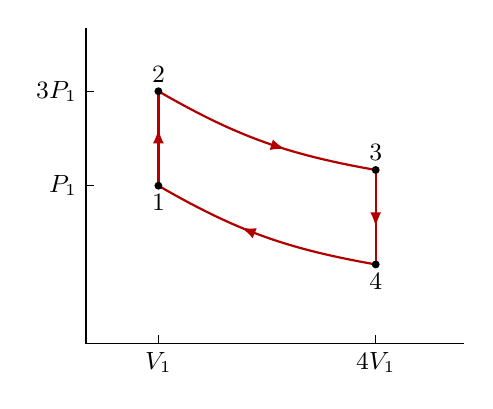
\begin{tikzpicture}\small
\def\L{4}\def\a{0.05}
\def\V{0.23*\L}
\draw (0,\L) -- (0,0) -- ({1.2*\L},0);
\coordinate (1) at ({\V},{0.5*\L});
\coordinate (2) at ({\V},{0.8*\L});
\coordinate (3) at ({4*\V},{0.55*\L});
\coordinate (4) at ({4*\V},{0.25*\L});
\draw[middlearrow,thick,red!70!black] (1) -- (2);
\draw[middlearrow,thick,red!70!black] (2) to[out=330,in=170] (3);
\draw[middlearrow,thick,red!70!black] (3) -- (4);
\draw[middlearrow,thick,red!70!black] (4) to[out=170,in=330] (1);
\fill (1) circle (\a) node[below] {$1$};
\fill (2) circle (\a) node[above] {$2$};
\fill (3) circle (\a) node[above] {$3$};
\fill (4) circle (\a) node[below] {$4$};
\draw ({\V},0) -- ++(0,0.1) node[pos=0,below]{$V_1$};
\draw ({4*\V},0) -- ++(0,0.1) node[pos=0,below]{$4V_1$};
\draw (0,{0.5*\L}) -- ++(0.1,0) node[pos=0,left]{$P_1$};
\draw (0,{0.8*\L}) -- ++(0.1,0) node[pos=0,left]{$3P_1$};
\end{tikzpicture}
\end{center}

\begin{parts}
\part\ssh\ $\dfrac{T_2}{T_1}$, $\dfrac{T_3}{T_1}$, $\dfrac{T_4}{T_1}$을 각각 구하시오. [8점]\\[13em]
\part\ssh\ $\dfrac{P_3}{P_1}$, $\dfrac{P_4}{P_1}$을 각각 구하시오. [6점]\\[13em]
\part\ddh\ 기관의 효율은 얼마인가? [4점]
\end{parts}

\vspace*{\fill}
\columnbreak

\question 그림과 같이 기전력 $\mathscr{E}$, 저항 $R_1$, $R_2$, $R_3$, 유도기 $L$, 스위치 $\mathrm{S}$로 구성된 회로가 있다. 물음에 답하시오. [총 15점]

\begin{center}
\ctikzset{bipoles/length=1cm}
\def\w{2.5}
\begin{circuitikz}\small
\draw (0,\w) to [battery1] (0,0); \node[left=0.3cm] at (0,{0.5*\w}) {$\mathcal{E}$};
\draw (0,\w) to [switch=$\mathrm{S}$] ({0.4*\w},\w) to [R=$R_1$] (\w,\w) to [R=$R_2$] (\w,0) to (0,0);
\draw (\w,\w) to [R=$R_3$] ({1.6*\w},\w) to [L=$L$] ({1.6*\w},0) to (\w,0);
\draw[-latex] ({0.5*\w},{0.9*\w}) -- ({0.9*\w},{0.9*\w}) node[pos=0.5,below]{$I_1$};
\draw[-latex] ({0.9*\w},{0.7*\w}) -- ({0.9*\w},{0.3*\w}) node[pos=0.5,left]{$I_2$};
\end{circuitikz}
\end{center}

\begin{parts}
\part \ssh\ 스위치 $\mathrm{S}$가 닫힌 직후 $I_1$과 $I_2$의 값을 각각 구하시오. (단 전류가 그림에 표시한 화살표 방향이면 양으로, 화살표 반대 방향이면 음으로 정한다.) [5점]\\[13em]
\part \ssh\ 시간이 충분히 많이 흘렀을 때 $I_1$과 $I_2$의 값을 각각 구하시오. [5점]\\[13em]
\part \ssh\ 그 후 다시 $\mathrm{S}$를 열었을 때의 $I_1$과 $I_2$의 값을 각각 구하시오. [5점]
\end{parts}

\vspace*{\fill}
\columnbreak

\question 한 변의 길이가 $L_x =L_y =L_z =L$인 상자 안에 질량 $m$인 입자가 하나 있다. [총 15점]
\begin{parts}
\part \ssh\ 입자의 바닥 상태의 에너지를 구하시오. [4점]\\[13em]
\part \ssh\ 두 번째 들뜬 상태의 에너지와 세 번째 들뜬 상태의 에너지 차이를 구하시오. [5점]\\[13em]
\part \ssh\ 첫 번째 들뜬 상태의 겹친 상태의 수와 다섯 번째 들뜬 상태의 겹친 상태의 수를 각각 구하시오. [6점]
\end{parts}


\vspace*{\fill}
\columnbreak

\question\nsh\ 쌍둥이 알버트와 발버트는 당연히 지구에서 같은 나이였다. 알버트가 지구에 머무는 동안 발버트는 15광년 떨어진 별까지 $0.6c$의 일정한 속력으로 갔다가 지체없이 동일한 속력으로 되돌아왔다.
\begin{center}
\includegraphics[width=0.4\columnwidth,frame]{./figures/twinparadox1.pdf}
\hspace{2em}
\includegraphics[width=0.4\columnwidth,frame]{./figures/twinparadox2.pdf}
\end{center}
알버트는 발버트의 시간이 자신의 시간보다 느리게 간다고 관찰하였고, 발버트는 알버트의 시간이 자신의 시간보다 느리게 간다고 관찰하였다. 둘이 지구에서 다시 만났을 때, 누가 얼마나 더 늙었는가? Minkowski diagram을 사용하여 설명하시오. [15점]




\end{questions}
\end{multicols*}



\end{document}